\section{Theoretical backgrounds}
\subsection{Nuclear spin}
Assuming a particles bescribed by its wavefunction $\Psi$, we can describe 
its fundamental properties by quantum numbers corrisponding to eigenstates
of different operators. Aside from the quantum number $n$ corresponding to the 
Hamiltonian $\hat{H}$ and thus to the energy level, particles can be further characterized 
by the orbital angular momentum quantum number $l$ and the spin quantum number 
$s$ as well as the projections of tboth of them onto the $z$-axis, given by 
$m_l$ and $m_s$, respectively. For the nucleus with wavefunction $\Psi_N$, 
spin and angular momentum are coupled to the 
nuclear spin with corresponding operator $\hat{I}$. Its properties are given by:
\begin{align}
    \hat{I} \Psi_N &= \mathbf{I} \Psi_N \\ 
\intertext{for which}
    \mathbf{I}^2 &= \hbar^2 I(I + 1)  &\text{(absolute value)} \\
    \left[\hat{H}, \hat{I}^2\right]_- &= 0  &\text{(constant)}
\end{align}
For the quantum number of nuclear spin, we have $I \in {0, \frac{1}{2}, 1, \ldots}$, while $\hbar$ is the 
reduced Planck constant. A second constant quantum number corresponding to the nuclear spin can be defined:
the projection on the $z$-axis, which in the experiment is given by the direction of the external $B$-field.
It is given by
\begin{align}
    I_z &= m_I \hbar \\
    m_I &\in \left\{-I, -I + 1, \ldots, I - 1, I\right\}
\end{align}
Thus, we have $2I + 1$ values for $m_I$. Depending on whether $I$ is integer or half integer, 
we have to apply Bose- or Fermi-statistics; the particles are called bosons or fermions, 
accordingly~\cite{Demtroeder1}.

\subsection{Magnetic moment}
Magnetic moment
\begin{equation}
    \mathbf{\mu} \mu = \gamma_K \mathbf{I}
\end{equation}
unit: \emph{nuclear magnetcon}
\begin{equation}
    \mu_K = \frac{\hbar e}{2 m_p}
\end{equation}


\subsection{Nuclear magnetic resonance}
\subsection{Relaxation}

\subsection{Hall effect and sensor}

\subsection{Lock-in method}
In order to supress noise and frequencies from other processes, we use
a frequently used method called ``lock-in amplification''. Depending on your
setup it is possible to reduce the noise by a factor $10^6$. The method
is based on the orthogonality relation of sinusoidal functions (which
can be seen easily if you differentiate the left with respect to $x$):
\begin{equation}
    \int \sin(a x) \sin(b x) dx =\frac{ b \sin(a x) \cos(b x)-a \cos(a x)
            \sin(b x)}{a^2-b^2}
\end{equation}
If we let the integration go from $\infty$ to $-\infty$ we end up with:
\begin{equation}
    (a,b) := \int_{-\infty}^{\infty} \sin(a x) \sin(b x) dx = \delta(a - b)
\end{equation}
Which stems from the sinusoidal functions forming a complete basis with
the integral as inner product.
Since we cannot use the integral over the whole real line, we have to rely
on shorter times: 
\begin{equation}
    (a,b)_t := \int_{0}^{t} \sin(a x) \sin(b x) dx = \delta(a - b)
\end{equation}
\paragraph{case 1: $t = 2k\pi /a$:}
\begin{equation}
    (a,b)_{2\pi /a} = \frac{a \sin(2\pi k\frac{a}{b})}{b^2 - a^2}
\end{equation}
\paragraph{case 1: $t = 2k\pi /b$:}
\begin{equation}
    (a,b)_{2\pi /b} = \frac{b \sin(2\pi k\frac{a}{b})}{a^2 - b^2}
\end{equation}
We notice we can distinguish whether the frequencies are equal or not 
since there is a singularity, but with restrictions:
\begin{itemize}
    \item The integral is evaluated continuosly, which is not possible
        in the real case, so the singularity is replaced by peak, which
        has a finite width.
\item As we do not integrate over the whole real line, we see in the two
    cases that higher harmonics (when working with nonlinear phenomena)
    can appear as well, which should be taken into account.
\item The strength which discriminates the $a=b$ from the $a\neq b$ case
    (the effective bandwidth)
    depends on the Ampitude of the reference signal. 
\end{itemize}

Now we can 
use in such a way that we take the input signal, multiply it by a
reference signal and integrate the result over a given time.
We chose the reference signal with a frequency in the range where we
expect our signal frequency to be: \\\\
\begin{tabular}{l|l}
    \textbf{Phase difference} & \textbf{Recieved Signal} \\
    \hline
    $0^\circ$ & maximal\\
    $180^{\circ}$ & minimal \\
    $90^\circ$ or $270^\circ$ & 0 
\end{tabular}
\vspace{0.5cm}\\\\
In our experiment we use as a reference signal a sawtooth curve, modulated
with a sinus:
\begin{equation}
   U(t) = U_{sz} \left[ t - \lfloor t \rfloor \,  \right] + U_0 \sin(\omega t)
\end{equation}
where the $\lfloor t \rfloor$ denotes to the gauss bracket (rounding up). 
\begin{figure}[htpb]
    \centering
    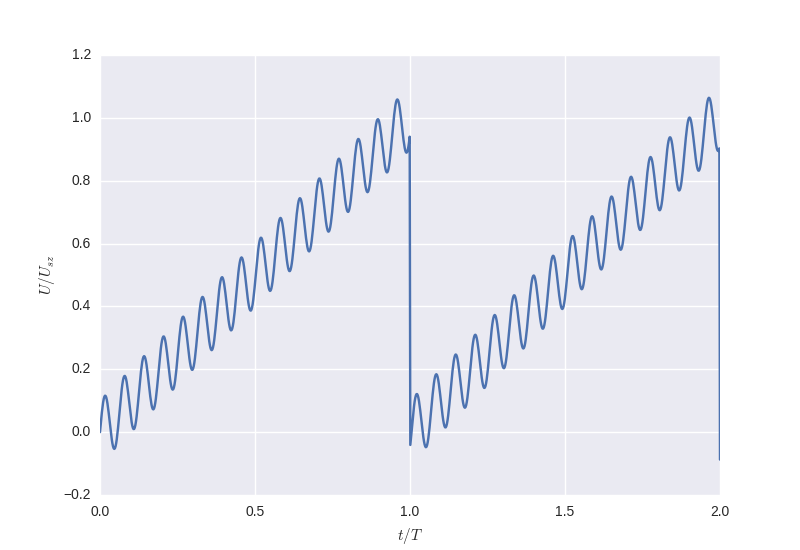
\includegraphics[width=0.8\linewidth]{figures/sawtooth}
    \caption{Reference signal for our lockin amplifier}
    \label{fig:sawtooth}
\end{figure}


\subsection{Materiales used in the experiment}

(PTFE, know by the brand name Teflon), 
